%!TEX root = skripsi.tex
%-----------------------------------------------------------------------------%
\chapter{\babSatu}
%-----------------------------------------------------------------------------%


%-----------------------------------------------------------------------------%
\section{Background}
%-----------------------------------------------------------------------------%
	
Semantic Role Labeling (SRL) is a task in Natural Language Processing (NLP) which aims to automatically assign semantic roles to each argument for each predicate in a given input sentence~\citep{jurafsky2016speech}. As for a brief definition, given an input sentence, SRL system will give an output of \textit{"Who did what to whom"} with \textit{what} as the predicate and \textit{who} and \textit{whom} being the argument of the predicate. SRL is an integral part of understanding natural language as it helps the machine to retrieve semantic information from the input. In practice, SRL has been widely used as one of the intermediate steps for many NLP tasks, some of which are information extraction~\citep{emanuele2013textual, surdeanu2003using}, machine translation~\citep{liu2010semantic, lo2013improving}, and question-answering~\citep{shen2007using, moschitti2003open}.

A chat bot system consists of three steps as shown in Figure~\ref{fig:botpipeline}, starting from understanding the incoming message from a user using Natural Language Understanding (NLU) system, tracking the dialogue using Dialogue State Tracking (DST), and finally generating a response using Natural Language Generation (NLG) system.

\begin{figure}
	\centering
	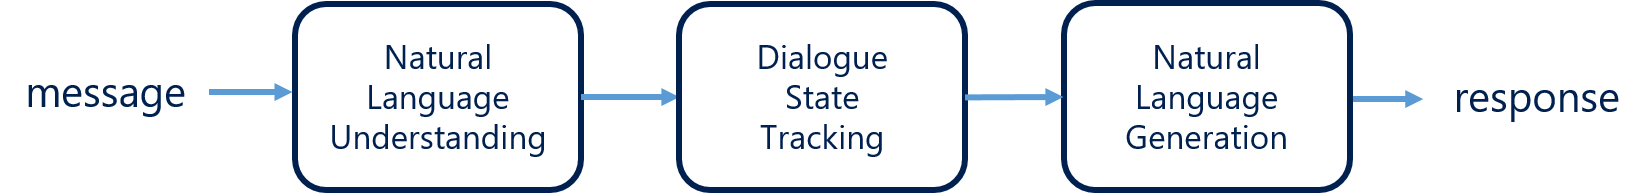
\includegraphics[width=1.0\linewidth]{images/botpipeline2}
	\caption{Chat bot system pipeline}
	\label{fig:botpipeline}
\end{figure}

In the chat bot system, SRL can be a useful part of the chat bot pipeline under the NLU step in order to extract the semantic representation of the user's text. To illustrate, suppose that the user sends a message to the chat bot for ordering a food as presented bellow.
\\
\\
\texttt{\textbf{Input:} 
	\textit{"Please buy me a burger at 1 PM"}}
\\

Using the SRL system under NLU pipeline, the chatbot system extracts the semantic information of the chat as follows.
\\
\\
\texttt{\textbf{Roles:}}

\texttt{Predicate: \textit{buy}}

\texttt{Patient: \textit{burger}}

\texttt{Beneficiary: \textit{me}}

\texttt{When: \textit{12 PM}}
\\

The system detects that the predicate is \textit{"buy"}, followed by \textit{"burger"} as the patient, or the thing being bought. The beneficiary, or the recipient, is \textit{"me"}. Lastly, the time is \textit{"12 AM"}. With this information, the bot can track the required information using DST to find the missing information of the order such as the flavor of the burger and the restaurant to buy it. After that, the bot can then processes the order to buy the burger for the user, followed by replying the user with a response using NLG system.

%the bots need to understand semantic information of the user's text in order to generate more personalized response. To illustrate, suppose that the user send a text chat to the bot and the SRL system extracts the semantic roles as presented bellow.
%\\
%
%\texttt{\textbf{Input:} 
%\textit{"I just ate chicken rice! Haha"}}
%
%\texttt{\textbf{Roles:}}
%
%\texttt{Predicate: \textit{eat}}
%
%\texttt{Agent: \textit{I}}
%
%\texttt{Patient: \textit{chicken rice}}
%\\
%
%By knowing that the user just ate a chicken rice, the bot can thus response with \textit{"That's great! how was the chicken?"}. This way, the user will be more engaged to the conversation with the bot.

SRL has been extensively studied for English formal language. Most of the traditional SRL systems are built based on language-dependent features such as syntactic parsers~\citep{gildea2002automatic, gildea2002necessity, pradhan2005semantic}. This syntactic information plays a pivotal role in solving SRL problem for traditional systems as it addresses SRL's long distance dependency~\citep{zhou2015end}. Unfortunately, this approach hardly depends on the linguistic experts experience assigning the correct syntactic information to the training data, which is costly~\citep{zhou2015end}. Moreover, if we want to build such system for another language, we have to define the syntactic information all over again~\citep{zhou2015end}. In order to address such problem, ~\cite{zhou2015end} proposed an end-to-end learning of SRL using Recurrent Neural Networks (RNN). In their research, they used Deep Bi-Directional Long Short-Term Memory (DB-LSTM) as the approach for RNN. The advantage of their system is that it only needs words of sentences as the input feature, and does not need any syntactic parsing since LSTM approach addresses the long distance relationship property of SRL problem. The research result outperforms the previous state-of-the-art traditional SRL systems as it achieved an F1 score of 81,07\%. One of other works involving deep learning for SRL is done by~\cite{collobert2011natural} who used Convolutional Neural Networks (CNN) as the main architecture.

On the other hand, the number of research focusing on SRL for Indonesian language (next, will be called as \textit{Indonesian}) is still low. One example would be a research done by~\cite{skripsidewi}, which proposed SRL for Indonesian using Support Vector Machine. They used the TreeBank data (in English) translated to Indonesian language using Google Translate. The research result opens a window of improvement as the best result consists of 61,6\% precision and 66,8\% recall. Another work focusing on SRL for Indonesian was done~\cite{skripsinur}, which used case grammar theory for SRL. However, the research concludes that not all sentences could be labeled as it did not cover all types of verbs in Indonesian. These facts open an opportunity to explore a more robust approach for Indonesian SRL as well as the need for a more reliable data.

This research is supported by Kata.ai, a technology company focusing on Artificial Intelligence (AI) and NLP development in Indonesian language. Its goal is to empower businesses by leveraging the power of AI and NLP towards customer engagement in a form of chat-bot. In order to achieve it, there has been an ongoing research project by the company focusing on Indonesian NLP. Since it uses chatting platforms as the medium, the scope of the project is for Indonesian conversational language. Conversational language is the most natural way people use to communicate in their daily life and thus, it is important to understand the language better through SRL.

Telling from the characteristics, Indonesian conversational language has its own challenges. It has many slang words for daily conversations. For example, the verb 'belikan' ('buy') has its informal form which is 'beliin'. Another example would be 'berbicara' ('talk') as 'ngobrol'. It happens to many words in Indonesian. Not to mention the variety of ways to express pronoun 'aku' ('I') such as 'gw', 'gue', and 'aq'. Yet, they have many kinds of interjection such as 'eh', 'duuh', 'dong', 'kok' which complexify the sentence structure. Moreover, the grammars of conversational language are often unstructured. These are the challenges that the SRL system should tackle in dealing with Indonesian conversational language.

Based on the fact that we still lack Indonesian SRL research, it is an interesting opportunity to build SRL system for Indonesian. Moreover, there is an industrial need from Kata.ai for understanding Indonesian conversational language. Our main contribution in this work is solving SRL problem on Indonesian conversational language. We will deep dive into the semantic role characteristics found in the language. After that, we will use deep learning as the state-of-the-art approach that has been emerging in NLP field for doing the SRL task. There is a wide variety of features and model architectures that can be used to train the SRL model. It is thus important for us to find the best feature combinations and model architecture for solving SRL on Indonesian conversational language.
%While many of the previous works studied SRL on formal language, our research aims to explore SRL on conversational language, which is still under-resourced. Following Zhou et al.~\cite{zhou2015end}, we view SRL as a sequence labeling problem. We thus introduce a new set of semantic roles for this language type. Furthermore, we propose a new architecture named Context-Aware Bi-Directional Long Short-Term Memories, designed with attention mechanism in order to capture context information of the sentence at a higher level.

%This work explores the SRL on conversational language, including creating a new set of semantic roles and proposing a new architecture, the so-called Context-Aware Bi-Directional Long Short-Term Memory Networks. We utilized word embedding and linguistic components as our main features. The SRL task was mainly evaluated on Indonesian conversational language used on chatting platform. Although this is a pilot task, we obtained a really promising result with F1 score of 74.78\%.

%-----------------------------------------------------------------------------%
\section{Problem Statement}
%-----------------------------------------------------------------------------%
Based on the motivation described in the background, the following problem statements are proposed:
\begin{enumerate}
	% Bagaimana --- %
	\item How to solve SRL for Indonesian conversational language with sequence labeling approach using deep learning? 
	\item Which feature combination outputs the best performance?
	\item Which deep learning model architecture gives the best result?
\end{enumerate}

%-----------------------------------------------------------------------------%
\section{Objectives and Contributions}
%-----------------------------------------------------------------------------%
%The objectives of this research includes understanding the semantic role characteristics of informal Indonesian short text and performing Semantic Role Labeling for informal Indonesian short text using deep learning approaches.
This research aims to build an SRL system for Indonesian conversational language. The main contributions of this work include creating a new set of semantic roles for Indonesian conversational language as well as proposing features and architectures for solving the SRL problem.

%-----------------------------------------------------------------------------%
\section{Methodology}
%-----------------------------------------------------------------------------%
The methodology of this work consists of literature review, data gathering, model development, experiment, evaluations and analysis, and conclusion.

\begin{enumerate}
	\item Literature Review\\
	In this step, we did a comprehensive study on Natural Language Processing (NLP) and Machine Learning (ML) aspects. The NLP aspect includes language model and semantic role labeling. For machine learning, we learned deep learning approaches such as recurrent neural networks and convolutional neural networks. These knowledge are the basis to support our research
	
	\item Data Gathering\\
	Since there seems to be no available corpus for SRL on Indonesian, especially conversational language, we annotated our own corpus. We retrieved the real word data from one of Kata.ai's chat bots. For this annotation, we build a new set of semantic roles crafted for Indonesian conversational language.
	
	\item Model Development\\
	After we gathered our corpus, we then design the model for the experiment in this research. We define the feature extractions and the deep learning model architecture that will be tested. In this section, we also propose our own architecture.
		
	\item Experiment \\
	In this step, we design our experiment scenarios. There are two set of scenarios consisting of feature and architecture experiments. The first one aims to find which feature combination outputs the best result, meanwhile the later focuses on finding the deep learning architecture that produces the highest performance.
	
	\item Evaluation and Analysis \\
	The experiment results are then to be evaluated and analyzed. We use precision, recall, and F1 as the metrics for the evaluation. We also conduct error analysis to get a deeper insight on the results.
	
	\item Conclusion \\
	In the end, we conclude our findings in our research based on the evaluations and analyses of the experiments. We then describe some future works that can be done following the results of this research.
\end{enumerate}

%-----------------------------------------------------------------------------%
%\section{Scope}
%We scope our research to these kinds of sentences:
%\begin{enumerate}
%	\item Single predicate in a form of verb.
%	\item Single predicate in a form of adjective.
%\end{enumerate}
%-----------------------------------------------------------------------------%

%-----------------------------------------------------------------------------%
\section{Organization}
%-----------------------------------------------------------------------------%
This report is organized as follows. In Chapter 2, literature review on the language models, deep learning architectures, and semantic role labeling will be shown. The methodology of this research is described in Chapter 3, including the features and the model architectures being used. This chapter will also provide the new idea of contribution for this research. In Chapter 4, the implementations of our methodology are described with the details of tools used and the measurement setup. The experiment scenarios, results, and analyses are presented in Chapter 5. Lastly, the conclusion and possible future works are described in Chapter 6.

%This report is organized as follows. We first explain the previous works on SRL systems in section 2. In section 3, the methodology of the research is described, . The results and analysis are then explained in section 4. Finally, we report our conclusion and potential future works in the last section.
%\begin{itemize}
%
%	\item Chapter 1 \babSatu \\
%	Pada bab ini \saya~menjelaskan mengenai motivasi dalam melakukan penelitian ini dan komponen-komponen utama penelitian seperi latar belakang, perumusan masalah, tujuan dan manfaat penelitian, metodologi penelitian, ruang lingkup penelitian dan sistematika penulisan.
%	
%	\item Chapter 2 \babDua \\
%	Pada bab ini \saya~melakukan studi literatur mengenai beberapa teori dan penelitian yang dilakukan oleh penulis lain. 
%		
%	\item Chapter 3 \babTiga \\
%	Pada bab ini \saya~menjelaskan alur dari penelitian ini, yaitu pengumpulan data, pra-pemrosesan, pelabelan, pengembangan model, eksperimen dan evaluasi.
%		
%	\item Chapter 4 \babEmpat \\
%	Pada bab ini \saya~menjelaskan proses implementasi sistem dan eksperimen berdasarkan rancangan yang telah \penulis~tentukan pada bab sebelumnya. Selain itu \saya~juga menjelaskan implementasi dari masing-masing tahapan yang dilakukan.
%		
%	\item Chapter 5 \babLima \\
%	Pada bab ini \saya~menjelaskan analisis dari hasil eksperimen yang telah \saya~kerjakan pada tahap sebelumnya. Hasil eksperimen \saya~sajikan dalam bentuk tabel dan grafik.
%	
%	\item Chapter 6 \babEnam \\
%	Pada bab ini \saya~memberikan kesimpulan berdasarkan hasil eksperimen dan analisis yang telah dilakukan pada penelitian ini. Selain itu \saya~juga memberikan saran dan masukan untuk penelitian dan pengembangan sistem mengenai \mer~berbahasa Indonesia selanjutnya.
%	
%\end{itemize}